\begin{figure}[t]
\centering
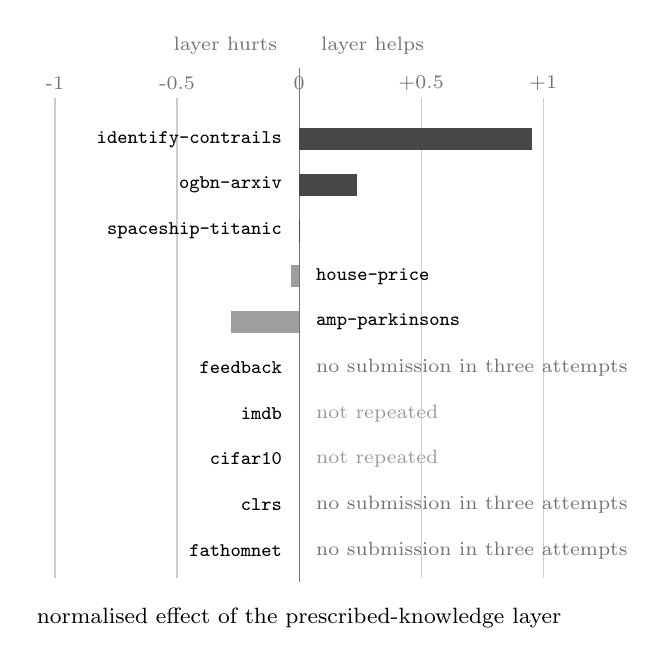
\begin{tikzpicture}[x=3.1cm,y=0.58cm]
\draw[black!55] (0,1.05) -- (0,-10.2);
\draw[black!20] (-1,0.4) -- (-1,-10.1);
\node[font=\scriptsize,black!55] at (-1,0.72) {-1};
\draw[black!20] (-0.5,0.4) -- (-0.5,-10.1);
\node[font=\scriptsize,black!55] at (-0.5,0.72) {-0.5};
\draw[black!20] (0.5,0.4) -- (0.5,-10.1);
\node[font=\scriptsize,black!55] at (0.5,0.72) {+0.5};
\draw[black!20] (1,0.4) -- (1,-10.1);
\node[font=\scriptsize,black!55] at (1,0.72) {+1};
\node[font=\scriptsize,black!55] at (0,0.72) {0};
\fill[black!72] (0,-0.74) rectangle (0.9551,-0.26);
\node[anchor=east,font=\scriptsize] at (-0.03,-0.5) {\texttt{identify-contrails}};
\fill[black!72] (0,-1.74) rectangle (0.2373,-1.26);
\node[anchor=east,font=\scriptsize] at (-0.03,-1.5) {\texttt{ogbn-arxiv}};
\fill[black!72] (0,-2.74) rectangle (0.0043,-2.26);
\node[anchor=east,font=\scriptsize] at (-0.03,-2.5) {\texttt{spaceship-titanic}};
\fill[black!38] (0,-3.74) rectangle (-0.0328,-3.26);
\node[anchor=west,font=\scriptsize] at (0.03,-3.5) {\texttt{house-price}};
\fill[black!38] (0,-4.74) rectangle (-0.2797,-4.26);
\node[anchor=west,font=\scriptsize] at (0.03,-4.5) {\texttt{amp-parkinsons}};
\node[font=\scriptsize,black!55,anchor=west] at (0.03,-5.5) {no submission in three attempts};
\node[anchor=east,font=\scriptsize] at (-0.03,-5.5) {\texttt{feedback}};
\node[font=\scriptsize,black!40,anchor=west] at (0.03,-6.5) {not repeated};
\node[anchor=east,font=\scriptsize] at (-0.03,-6.5) {\texttt{imdb}};
\node[font=\scriptsize,black!40,anchor=west] at (0.03,-7.5) {not repeated};
\node[anchor=east,font=\scriptsize] at (-0.03,-7.5) {\texttt{cifar10}};
\node[font=\scriptsize,black!55,anchor=west] at (0.03,-8.5) {no submission in three attempts};
\node[anchor=east,font=\scriptsize] at (-0.03,-8.5) {\texttt{clrs}};
\node[font=\scriptsize,black!55,anchor=west] at (0.03,-9.5) {no submission in three attempts};
\node[anchor=east,font=\scriptsize] at (-0.03,-9.5) {\texttt{fathomnet}};
\node[font=\footnotesize,anchor=north] at (0,-10.55){normalised effect of the prescribed-knowledge layer};
\node[font=\scriptsize,black!55,anchor=south east] at (-0.05,1.15) {layer hurts};
\node[font=\scriptsize,black!55,anchor=south west] at (0.05,1.15) {layer helps};
\end{tikzpicture}
\caption{The same layer, the same architecture, the same backbone, three attempts per cell: only the task changes. Two tasks gain, three lose outright---on those the treated branch exhausted its budget without submitting anything, three attempts out of three---and the rest are level. An aggregate over these tasks would report close to nothing while concealing that the layer costs three of them their entire result.}
\label{fig:signflip}
\end{figure}
